%%
% Copyright (c) 2017 - 2019, Pascal Wagler;  
% Copyright (c) 2014 - 2019, John MacFarlane
% 
% All rights reserved.
% 
% Redistribution and use in source and binary forms, with or without 
% modification, are permitted provided that the following conditions 
% are met:
% 
% - Redistributions of source code must retain the above copyright 
% notice, this list of conditions and the following disclaimer.
% 
% - Redistributions in binary form must reproduce the above copyright 
% notice, this list of conditions and the following disclaimer in the 
% documentation and/or other materials provided with the distribution.
% 
% - Neither the name of John MacFarlane nor the names of other 
% contributors may be used to endorse or promote products derived 
% from this software without specific prior written permission.
% 
% THIS SOFTWARE IS PROVIDED BY THE COPYRIGHT HOLDERS AND CONTRIBUTORS 
% "AS IS" AND ANY EXPRESS OR IMPLIED WARRANTIES, INCLUDING, BUT NOT 
% LIMITED TO, THE IMPLIED WARRANTIES OF MERCHANTABILITY AND FITNESS 
% FOR A PARTICULAR PURPOSE ARE DISCLAIMED. IN NO EVENT SHALL THE 
% COPYRIGHT OWNER OR CONTRIBUTORS BE LIABLE FOR ANY DIRECT, INDIRECT, 
% INCIDENTAL, SPECIAL, EXEMPLARY, OR CONSEQUENTIAL DAMAGES (INCLUDING,
% BUT NOT LIMITED TO, PROCUREMENT OF SUBSTITUTE GOODS OR SERVICES; 
% LOSS OF USE, DATA, OR PROFITS; OR BUSINESS INTERRUPTION) HOWEVER 
% CAUSED AND ON ANY THEORY OF LIABILITY, WHETHER IN CONTRACT, STRICT 
% LIABILITY, OR TORT (INCLUDING NEGLIGENCE OR OTHERWISE) ARISING IN 
% ANY WAY OUT OF THE USE OF THIS SOFTWARE, EVEN IF ADVISED OF THE 
% POSSIBILITY OF SUCH DAMAGE.
%%

%%
% This is the Eisvogel pandoc LaTeX template.
%
% For usage information and examples visit the official GitHub page:
% https://github.com/Wandmalfarbe/pandoc-latex-template
%%

\PassOptionsToPackage{unicode=true}{hyperref} % options for packages loaded elsewhere
\PassOptionsToPackage{hyphens}{url}
\PassOptionsToPackage{dvipsnames,svgnames*,x11names*,table}{xcolor}
%
\documentclass[
  10pt,
  english,
  letterpaper,
,tablecaptionabove
]{scrartcl}
\usepackage{lmodern}
\usepackage{setspace}
\setstretch{1.2}
\usepackage{amssymb,amsmath}
\usepackage{ifxetex,ifluatex}
\ifnum 0\ifxetex 1\fi\ifluatex 1\fi=0 % if pdftex
  \usepackage[T1]{fontenc}
  \usepackage[utf8]{inputenc}
  \usepackage{textcomp} % provides euro and other symbols
\else % if luatex or xelatex
  \usepackage{unicode-math}
  \defaultfontfeatures{Scale=MatchLowercase}
  \defaultfontfeatures[\rmfamily]{Ligatures=TeX,Scale=1}
\fi
% use upquote if available, for straight quotes in verbatim environments
\IfFileExists{upquote.sty}{\usepackage{upquote}}{}
\IfFileExists{microtype.sty}{% use microtype if available
  \usepackage[]{microtype}
  \UseMicrotypeSet[protrusion]{basicmath} % disable protrusion for tt fonts
}{}
\makeatletter
\@ifundefined{KOMAClassName}{% if non-KOMA class
  \IfFileExists{parskip.sty}{%
    \usepackage{parskip}
  }{% else
    \setlength{\parindent}{0pt}
    \setlength{\parskip}{6pt plus 2pt minus 1pt}}
}{% if KOMA class
  \KOMAoptions{parskip=half}}
\makeatother
\usepackage{xcolor}
\definecolor{default-linkcolor}{HTML}{A50000}
\definecolor{default-filecolor}{HTML}{A50000}
\definecolor{default-citecolor}{HTML}{4077C0}
\definecolor{default-urlcolor}{HTML}{4077C0}
\IfFileExists{xurl.sty}{\usepackage{xurl}}{} % add URL line breaks if available
\IfFileExists{bookmark.sty}{\usepackage{bookmark}}{\usepackage{hyperref}}
\hypersetup{
  pdftitle={Graphs (Part 2)},
  pdfauthor={Connor Baker},
  pdfsubject={Graphs},
  pdfkeywords={Lecture, Graphs},
  pdfborder={0 0 0},
  breaklinks=true}
\urlstyle{same}  % don't use monospace font for urls
\usepackage[margin=2.5cm,includehead=true,includefoot=true,centering]{geometry}
\usepackage{listings}
\newcommand{\passthrough}[1]{#1}
\lstset{defaultdialect=[5.3]Lua}
\lstset{defaultdialect=[x86masm]Assembler}
\usepackage{longtable,booktabs}
% Allow footnotes in longtable head/foot
\IfFileExists{footnotehyper.sty}{\usepackage{footnotehyper}}{\usepackage{footnote}}
\makesavenoteenv{longtable}
\usepackage{graphicx,grffile}
\makeatletter
\def\maxwidth{\ifdim\Gin@nat@width>\linewidth\linewidth\else\Gin@nat@width\fi}
\def\maxheight{\ifdim\Gin@nat@height>\textheight\textheight\else\Gin@nat@height\fi}
\makeatother
% Scale images if necessary, so that they will not overflow the page
% margins by default, and it is still possible to overwrite the defaults
% using explicit options in \includegraphics[width, height, ...]{}
\setkeys{Gin}{width=\maxwidth,height=\maxheight,keepaspectratio}
\setlength{\emergencystretch}{3em}  % prevent overfull lines
\providecommand{\tightlist}{%
  \setlength{\itemsep}{0pt}\setlength{\parskip}{0pt}}
\setcounter{secnumdepth}{-\maxdimen} % remove section numbering
% Redefines (sub)paragraphs to behave more like sections
\ifx\paragraph\undefined\else
  \let\oldparagraph\paragraph
  \renewcommand{\paragraph}[1]{\oldparagraph{#1}\mbox{}}
\fi
\ifx\subparagraph\undefined\else
  \let\oldsubparagraph\subparagraph
  \renewcommand{\subparagraph}[1]{\oldsubparagraph{#1}\mbox{}}
\fi

% Make use of float-package and set default placement for figures to H
\usepackage{float}
\floatplacement{figure}{H}

\setcounter{page}{0}
\lstset{breaklines=true}
\lstset{postbreak=\raisebox{0ex}[0ex][0ex]{\ensuremath{\color{blue}\hookrightarrow\space}}}
\usepackage{datetime}
\settimeformat{ampmtime}
\usepackage{lastpage}
\ifnum 0\ifxetex 1\fi=0 % if pdftex or luatex
  \usepackage[shorthands=off,main=english]{babel}
\else % if xetex
    % See issue https://github.com/reutenauer/polyglossia/issues/127
  \renewcommand*\familydefault{\sfdefault}
    % load polyglossia as late as possible as it *could* call bidi if RTL lang (e.g. Hebrew or Arabic)
  \usepackage{polyglossia}
  \setmainlanguage[]{english}
\fi

\title{Graphs (Part 2)}
\usepackage{etoolbox}
\makeatletter
\providecommand{\subtitle}[1]{% add subtitle to \maketitle
  \apptocmd{\@title}{\par {\large #1 \par}}{}{}
}
\makeatother
\subtitle{Graph representations and algorithms that operate on graphs}
\author{Connor Baker}
\date{2019-03-26, Compiled on \today~at \currenttime}





%%
%% added
%%

%
% language specification
%
% If no language is specified, use English as the default main document language.
%


%
% for the background color of the title page
%
\usepackage{pagecolor}
\usepackage{afterpage}

%
% TOC depth and 
% section numbering depth
%
\setcounter{tocdepth}{3}

%
% break urls
%
\PassOptionsToPackage{hyphens}{url}

%
% When using babel or polyglossia with biblatex, loading csquotes is recommended 
% to ensure that quoted texts are typeset according to the rules of your main language.
%
\usepackage{csquotes}

%
% captions
%
\definecolor{caption-color}{HTML}{777777}
\usepackage[font={stretch=1.2}, textfont={color=caption-color}, position=top, skip=4mm, labelfont=bf, singlelinecheck=false, justification=raggedright]{caption}
\setcapindent{0em}

%
% blockquote
%
\definecolor{blockquote-border}{RGB}{221,221,221}
\definecolor{blockquote-text}{RGB}{119,119,119}
\usepackage{mdframed}
\newmdenv[rightline=false,bottomline=false,topline=false,linewidth=3pt,linecolor=blockquote-border,skipabove=\parskip]{customblockquote}
\renewenvironment{quote}{\begin{customblockquote}\list{}{\rightmargin=0em\leftmargin=0em}%
\item\relax\color{blockquote-text}\ignorespaces}{\unskip\unskip\endlist\end{customblockquote}}

%
% Source Sans Pro as the de­fault font fam­ily
% Source Code Pro for monospace text
%
% 'default' option sets the default 
% font family to Source Sans Pro, not \sfdefault.
%
\usepackage[default]{sourcesanspro}
\usepackage{sourcecodepro}

% XeLaTeX specific adjustments for straight quotes: https://tex.stackexchange.com/a/354887
% This issue is already fixed (see https://github.com/silkeh/latex-sourcecodepro/pull/5) but the 
% fix is still unreleased.
% TODO: Remove this workaround when the new version of sourcecodepro is released on CTAN.
\ifxetex
\makeatletter
\defaultfontfeatures[\ttfamily]
  { Numbers   = \sourcecodepro@figurestyle,
    Scale     = \SourceCodePro@scale,
    Extension = .otf }
\setmonofont
  [ UprightFont    = *-\sourcecodepro@regstyle,
    ItalicFont     = *-\sourcecodepro@regstyle It,
    BoldFont       = *-\sourcecodepro@boldstyle,
    BoldItalicFont = *-\sourcecodepro@boldstyle It ]
  {SourceCodePro}
\makeatother
\fi

%
% heading color
%
\definecolor{heading-color}{RGB}{40,40,40}
\addtokomafont{section}{\color{heading-color}}
% When using the classes report, scrreprt, book, 
% scrbook or memoir, uncomment the following line.
%\addtokomafont{chapter}{\color{heading-color}}

%
% variables for title and author
%
\usepackage{titling}
\title{Graphs (Part 2)}
\author{Connor Baker}

%
% tables
%

\definecolor{table-row-color}{HTML}{F5F5F5}
\definecolor{table-rule-color}{HTML}{999999}

%\arrayrulecolor{black!40}
\arrayrulecolor{table-rule-color}     % color of \toprule, \midrule, \bottomrule
\setlength\heavyrulewidth{0.3ex}      % thickness of \toprule, \bottomrule
\renewcommand{\arraystretch}{1.3}     % spacing (padding)

% Reset rownum counter so that each table
% starts with the same row colors.
% https://tex.stackexchange.com/questions/170637/restarting-rowcolors
\let\oldlongtable\longtable
\let\endoldlongtable\endlongtable
\renewenvironment{longtable}{
\rowcolors{3}{}{table-row-color!100}  % row color
\oldlongtable} {
\endoldlongtable
\global\rownum=0\relax}

% Unfortunately the colored cells extend beyond the edge of the 
% table because pandoc uses @-expressions (@{}) like so: 
%
% \begin{longtable}[]{@{}ll@{}}
% \end{longtable}
%
% https://en.wikibooks.org/wiki/LaTeX/Tables#.40-expressions

%
% remove paragraph indention
%
\setlength{\parindent}{0pt}
\setlength{\parskip}{6pt plus 2pt minus 1pt}
\setlength{\emergencystretch}{3em}  % prevent overfull lines

%
%
% Listings
%
%


%
% listing colors
%
\definecolor{listing-background}{HTML}{F7F7F7}
\definecolor{listing-rule}{HTML}{B3B2B3}
\definecolor{listing-numbers}{HTML}{B3B2B3}
\definecolor{listing-text-color}{HTML}{000000}
\definecolor{listing-keyword}{HTML}{435489}
\definecolor{listing-identifier}{HTML}{435489}
\definecolor{listing-string}{HTML}{00999A}
\definecolor{listing-comment}{HTML}{8E8E8E}
\definecolor{listing-javadoc-comment}{HTML}{006CA9}

\lstdefinestyle{eisvogel_listing_style}{
  language         = java,
  numbers          = left,
  xleftmargin      = 2.7em,
  framexleftmargin = 2.5em,
  backgroundcolor  = \color{listing-background},
  basicstyle       = \color{listing-text-color}\small\ttfamily{}\linespread{1.15}, % print whole listing small
  breaklines       = true,
  frame            = single,
  framesep         = 0.19em,
  rulecolor        = \color{listing-rule},
  frameround       = ffff,
  tabsize          = 4,
  numberstyle      = \color{listing-numbers},
  aboveskip        = -0.7em,
  belowskip        = 0.1em,
  abovecaptionskip = 0em,
  belowcaptionskip = 1em,
  keywordstyle     = \color{listing-keyword}\bfseries,
  classoffset      = 0,
  sensitive        = true,
  identifierstyle  = \color{listing-identifier},
  commentstyle     = \color{listing-comment},
  morecomment      = [s][\color{listing-javadoc-comment}]{/**}{*/},
  stringstyle      = \color{listing-string},
  showstringspaces = false,
  escapeinside     = {/*@}{@*/}, % Allow LaTeX inside these special comments
  literate         =
  {á}{{\'a}}1 {é}{{\'e}}1 {í}{{\'i}}1 {ó}{{\'o}}1 {ú}{{\'u}}1
  {Á}{{\'A}}1 {É}{{\'E}}1 {Í}{{\'I}}1 {Ó}{{\'O}}1 {Ú}{{\'U}}1
  {à}{{\`a}}1 {è}{{\'e}}1 {ì}{{\`i}}1 {ò}{{\`o}}1 {ù}{{\`u}}1
  {À}{{\`A}}1 {È}{{\'E}}1 {Ì}{{\`I}}1 {Ò}{{\`O}}1 {Ù}{{\`U}}1
  {ä}{{\"a}}1 {ë}{{\"e}}1 {ï}{{\"i}}1 {ö}{{\"o}}1 {ü}{{\"u}}1
  {Ä}{{\"A}}1 {Ë}{{\"E}}1 {Ï}{{\"I}}1 {Ö}{{\"O}}1 {Ü}{{\"U}}1
  {â}{{\^a}}1 {ê}{{\^e}}1 {î}{{\^i}}1 {ô}{{\^o}}1 {û}{{\^u}}1
  {Â}{{\^A}}1 {Ê}{{\^E}}1 {Î}{{\^I}}1 {Ô}{{\^O}}1 {Û}{{\^U}}1
  {œ}{{\oe}}1 {Œ}{{\OE}}1 {æ}{{\ae}}1 {Æ}{{\AE}}1 {ß}{{\ss}}1
  {ç}{{\c c}}1 {Ç}{{\c C}}1 {ø}{{\o}}1 {å}{{\r a}}1 {Å}{{\r A}}1
  {€}{{\EUR}}1 {£}{{\pounds}}1 {«}{{\guillemotleft}}1
  {»}{{\guillemotright}}1 {ñ}{{\~n}}1 {Ñ}{{\~N}}1 {¿}{{?`}}1
  {…}{{\ldots}}1 {≥}{{>=}}1 {≤}{{<=}}1 {„}{{\glqq}}1 {“}{{\grqq}}1
  {”}{{''}}1
}
\lstset{style=eisvogel_listing_style}

\lstdefinelanguage{XML}{
  morestring      = [b]",
  moredelim       = [s][\bfseries\color{listing-keyword}]{<}{\ },
  moredelim       = [s][\bfseries\color{listing-keyword}]{</}{>},
  moredelim       = [l][\bfseries\color{listing-keyword}]{/>},
  moredelim       = [l][\bfseries\color{listing-keyword}]{>},
  morecomment     = [s]{<?}{?>},
  morecomment     = [s]{<!--}{-->},
  commentstyle    = \color{listing-comment},
  stringstyle     = \color{listing-string},
  identifierstyle = \color{listing-identifier}
}

%
% header and footer
%
\usepackage{fancyhdr}

\fancypagestyle{eisvogel-header-footer}{
  \fancyhead{}
  \fancyfoot{}
  \lhead[2019-03-26]{Graphs (Part 2)}
  \chead[]{}
  \rhead[Graphs (Part 2)]{2019-03-26}
  \lfoot[\thepage~of \pageref{LastPage}]{Connor Baker}
  \cfoot[]{}
  \rfoot[Connor Baker]{\thepage~of \pageref{LastPage}}
  \renewcommand{\headrulewidth}{0.4pt}
  \renewcommand{\footrulewidth}{0.4pt}
}
\pagestyle{eisvogel-header-footer}

%%
%% end added
%%

\begin{document}

%%
%% begin titlepage
%%

\begin{titlepage}
\newgeometry{left=6cm}
\definecolor{titlepage-color}{HTML}{FFFFFF}
\newpagecolor{titlepage-color}\afterpage{\restorepagecolor}
\newcommand{\colorRule}[3][black]{\textcolor[HTML]{#1}{\rule{#2}{#3}}}
\begin{flushleft}
\noindent
\\[-1em]
\color[HTML]{0d47a1}
\makebox[0pt][l]{\colorRule[0d47a1]{1.3\textwidth}{2pt}}
\par
\noindent

{ \setstretch{1.4}
\vfill
\noindent {\huge \textbf{\textsf{Graphs (Part 2)}}}
\vskip 1em
{\Large \textsf{Graph representations and algorithms that operate on graphs}}
\vskip 2em
\noindent
{\Large \textsf{Connor Baker}
\vfill
}


\textsf{2019-03-26, Compiled on \today~at \currenttime}}
\end{flushleft}
\end{titlepage}
\restoregeometry

%%
%% end titlepage
%%



\hypertarget{graphs-part-2}{%
\section{Graphs (Part 2)}\label{graphs-part-2}}

\hypertarget{road-map}{%
\subsection{Road Map}\label{road-map}}

\begin{itemize}
\tightlist
\item
  Graph basics

  \begin{itemize}
  \tightlist
  \item
    Definitions and terms
  \item
    Applications
  \end{itemize}
\item
  Graph representations

  \begin{itemize}
  \tightlist
  \item
    Adjacency matrix
  \item
    Adjacency list
  \end{itemize}
\item
  Graph algorithms

  \begin{itemize}
  \tightlist
  \item
    Graph traversal
  \item
    Shortest path problem
  \item
    Many more
  \end{itemize}
\end{itemize}

\hypertarget{graph-representation}{%
\subsection{Graph Representation}\label{graph-representation}}

\begin{itemize}
\tightlist
\item
  \emph{Graph}: a set of vertices \(V\) and edges \(E\)
\item
  Representation: the way in which we store a graph in programs

  \begin{itemize}
  \tightlist
  \item
    Adjacency matrix: a 2D array \passthrough{\lstinline!A[n][n]!} where
    \(n = |V|\)

    \begin{itemize}
    \tightlist
    \item
      \passthrough{\lstinline!A[v][w]!} is the weight of \((v,w)\)
    \item
      \passthrough{\lstinline!A[v][w]!} is infinity if \(v,w\) is not in
      the graph
    \end{itemize}
  \item
    Adjacency list

    \begin{itemize}
    \tightlist
    \item
      A group of \(|V|\) linked lists
    \item
      List \passthrough{\lstinline!v!}: a list of all nodes \(w\) such
      that there is an edge \((v, w)\)
    \end{itemize}
  \end{itemize}
\end{itemize}

\hypertarget{adjacency-matrix}{%
\subsection{Adjacency Matrix}\label{adjacency-matrix}}

\begin{figure}
\centering
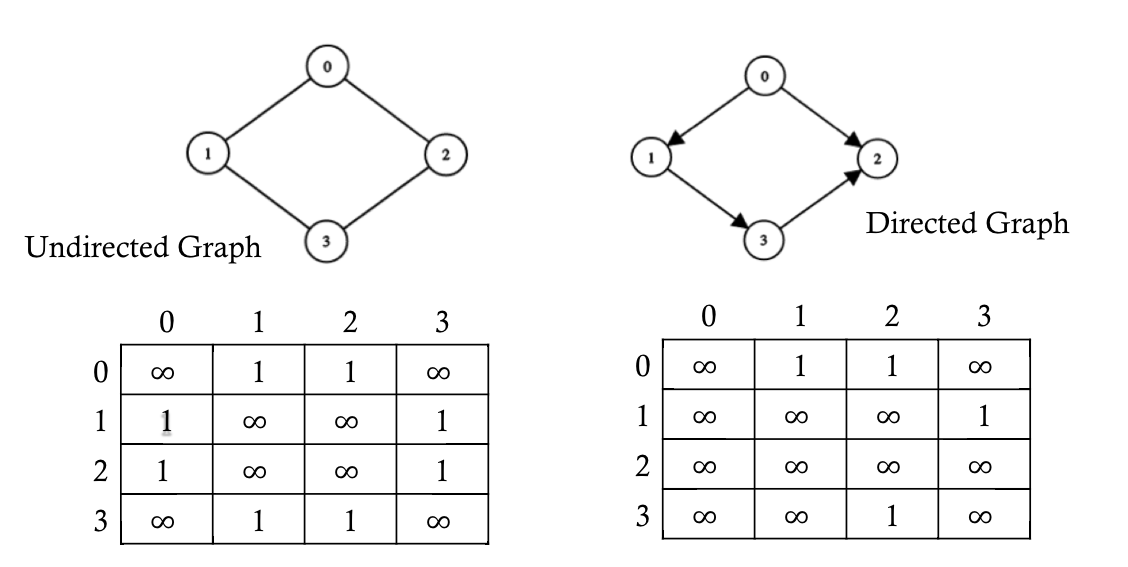
\includegraphics{images/1.png}
\caption{A comparison of features between undirected and directed
graphs}
\end{figure}

\hypertarget{adjacency-list}{%
\subsection{Adjacency List}\label{adjacency-list}}

Using the same image as above for reference, we have the following
adjacency lists:

\begin{itemize}
\tightlist
\item
  Undirected graph

  \begin{itemize}
  \tightlist
  \item
    \(0 \rightarrow 1 \rightarrow 2\)
  \item
    \(1 \rightarrow 0 \rightarrow 3\)
  \item
    \(2 \rightarrow 0 \rightarrow 3\)
  \item
    \(3 \rightarrow 1 \rightarrow 2\)
  \end{itemize}
\item
  Directed graph

  \begin{itemize}
  \tightlist
  \item
    \(0 \rightarrow 1 \rightarrow 2\)
  \item
    \(1 \rightarrow 3\)
  \item
    \(2 \rightarrow\) \passthrough{\lstinline!null!} (empty list)
  \item
    \(3 \rightarrow 2\)
  \end{itemize}
\end{itemize}

\hypertarget{complexity}{%
\subsection{Complexity}\label{complexity}}

\begin{itemize}
\tightlist
\item
  Adjacency matrix

  \begin{itemize}
  \tightlist
  \item
    Space cost: \(O(|V|^2)\)
  \item
    Initialization time: \(O(|V|^2)\)
  \item
    Fine with dense graphs, not so great for sparse ones
  \end{itemize}
\item
  Adjacency list

  \begin{itemize}
  \tightlist
  \item
    Space cost: \(O(|V| + |E|) = O(|E|)\)
  \item
    Initialization time: linear from a list of edges

    \begin{itemize}
    \tightlist
    \item
      Most cases, we skip the checking of duplicate edges (even though
      they might come with different edge weights)
    \end{itemize}
  \end{itemize}
\item
  How do we add, remove, or find a node or edge?
\end{itemize}

\hypertarget{graph-representation-example}{%
\subsection{Graph Representation
Example}\label{graph-representation-example}}

\begin{figure}
\centering
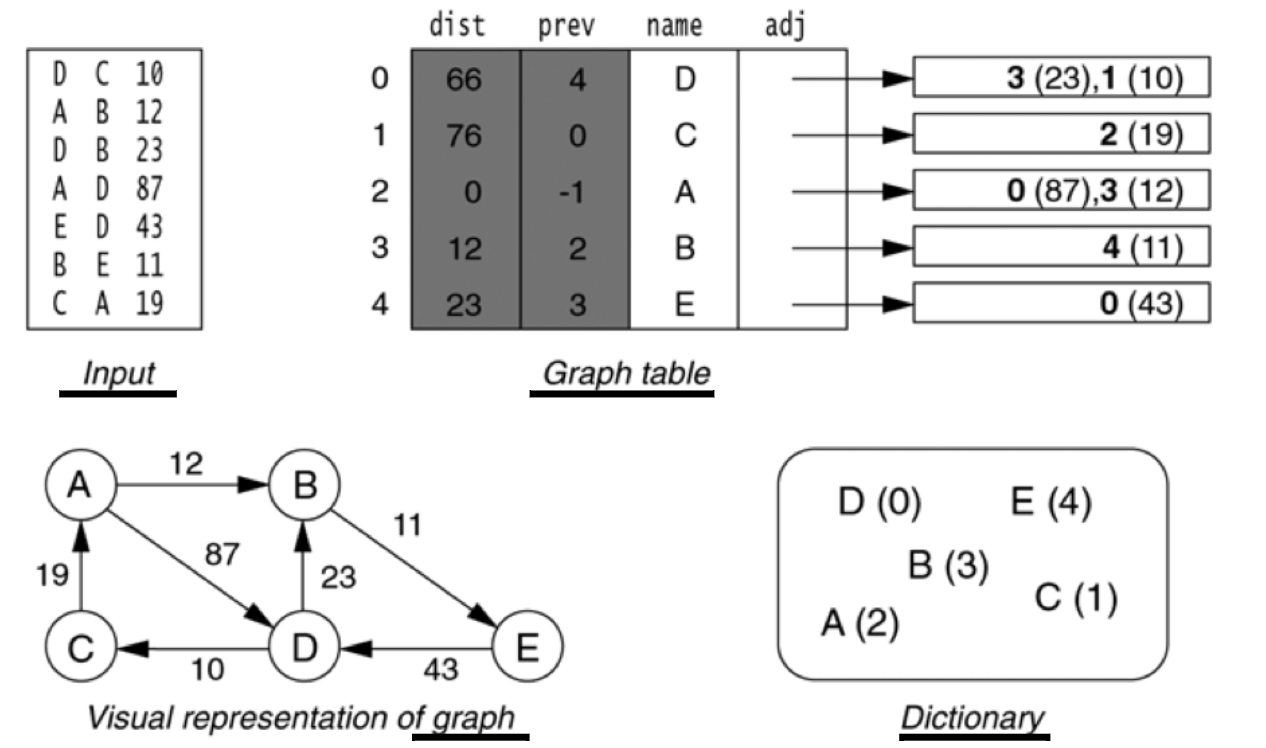
\includegraphics{images/2.png}
\caption{An abstract scenario of the data structures used in a
shortest-path calculation, with an input graph taken from a file. The
shortest weighted path from \passthrough{\lstinline!A!} to
\passthrough{\lstinline!C!} is \passthrough{\lstinline!A!} to
\passthrough{\lstinline!B!} to \passthrough{\lstinline!E!} to
\passthrough{\lstinline!D!} to \passthrough{\lstinline!C!} (cost is 76).
From Weiss, Figure 14.4}
\end{figure}

\hypertarget{graph-traversal-and-searching}{%
\subsection{Graph Traversal and
Searching}\label{graph-traversal-and-searching}}

\begin{itemize}
\tightlist
\item
  Basis of many graph algorithms
\item
  The general idea

  \begin{itemize}
  \tightlist
  \item
    Given a starting point, visit, check, or update every vertex in a
    graph by following the given edges
  \end{itemize}
\item
  Application examples

  \begin{itemize}
  \tightlist
  \item
    Connected components
  \item
    Topological sorting
  \item
    Minimum spanning tree (MST)
  \item
    Shortest path
  \item
    Many more
  \end{itemize}
\item
  Procedure

  \begin{itemize}
  \tightlist
  \item
    Given a starting point, visit, check, or update every vertex in a
    graph by following the given edges
  \item
    Order: which vertex do we visit next?
  \end{itemize}
\item
  Basic approaches

  \begin{itemize}
  \tightlist
  \item
    \emph{Breadth-first}: visit vertices in layers -- those closest to
    the start are visited first, and those most distant are visited last
  \item
    \emph{Depth-first}: from the starting vertex, explore as far as
    possible along each path before backtracking
  \item
    Remember tree traversals? They're baaaaaaack!
  \end{itemize}
\end{itemize}

\hypertarget{breadth-first-traversal}{%
\subsection{Breadth-First Traversal}\label{breadth-first-traversal}}

\begin{itemize}
\tightlist
\item
  Given the starting point \(S\)

  \begin{itemize}
  \tightlist
  \item
    Visit all the nodes that are one edge away (\(S\)'s direct
    neighbors)
  \item
    Visit all nodes that are two edges away (neighbors of neighbors)
  \item
    Visit all nodes that are three edges away (neighbors of neighbors of
    neighbors)
  \item
    \ldots{}
  \item
    Repeat this until all nodes have been visited
  \end{itemize}
\end{itemize}

\hypertarget{traversal-example-breadth-first}{%
\subsection{Traversal Example:
Breadth-First}\label{traversal-example-breadth-first}}

\begin{figure}
\centering
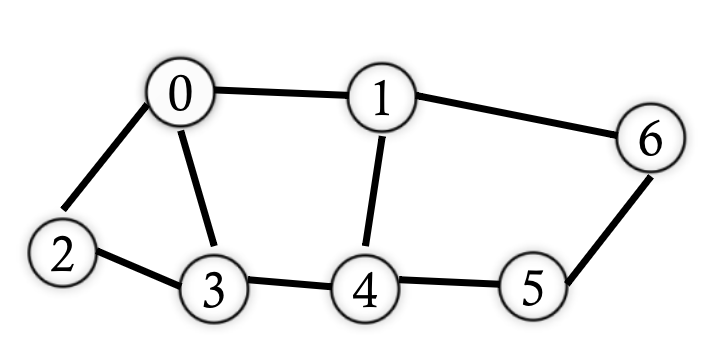
\includegraphics[width=0.5\textwidth,height=\textheight]{images/3.png}
\caption{Example 1}
\end{figure}

\begin{itemize}
\tightlist
\item
  A breadth-first traversal starting with \(0\): \(\{0\}\)

  \begin{itemize}
  \tightlist
  \item
    Visit all the nodes adjacent to \(0\): \(\{0, 1, 2, 3\}\)
  \item
    Visit all the neighbors of those nodes: \(\{0, 1, 2, 3, 4, 6\}\)
  \item
    Continue the process: \(\{0, 1, 2, 3, 4, 6, 5\}\)
  \item
    We've reached all the nodes, so we can stop. We've also found that
    every node in this graph can be reached by a path of at most length
    \(3\).
  \end{itemize}
\end{itemize}

\hypertarget{breadth-first-traversal-implementation}{%
\subsection{Breadth-First Traversal
Implementation}\label{breadth-first-traversal-implementation}}

\begin{itemize}
\tightlist
\item
  Have we done something similar to this before?

  \begin{itemize}
  \tightlist
  \item
    Yes, and depending on your progress in Project 3 you might still be
    doing it.
  \end{itemize}
\item
  We can use a queue

  \begin{itemize}
  \tightlist
  \item
    Initialize by enqueueing the starting vertex
  \item
    Mark it as visited when we enqueue
  \item
    Process the vertives in a first-in first-out (FIFO) order:

    \begin{itemize}
    \tightlist
    \item
      Dequeue the first vertex \(v\)
    \item
      Enqueue \(v\)'s neighbor that has not yet been visited or marked
    \end{itemize}
  \end{itemize}
\end{itemize}

\hypertarget{depth-first-traversal}{%
\subsection{Depth-First Traversal}\label{depth-first-traversal}}

\begin{itemize}
\tightlist
\item
  Given the starting point \(S\)

  \begin{itemize}
  \tightlist
  \item
    Visit the first neighbor of \(S\)
  \item
    Visit the first neighbor of the first neighbor of \(S\)
  \item
    Visit the first neighbor fo the first neighbor of the first neighbor
    of \(S\)
  \item
    Repeat this process until there are no more nodes to go, then back,
    trying the second neighbor of \(S\)
  \item
    Repeat that process until we've processed all of the neighbors of
    \(S\)
  \end{itemize}
\end{itemize}

\hypertarget{traversal-example-depth-first}{%
\subsection{Traversal Example:
Depth-First}\label{traversal-example-depth-first}}

\begin{figure}
\centering
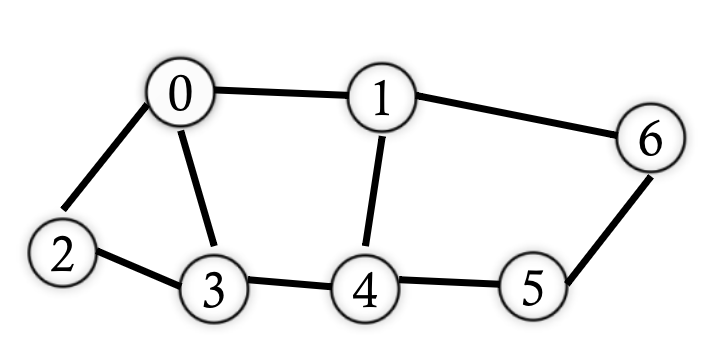
\includegraphics[width=0.5\textwidth,height=\textheight]{images/3.png}
\caption{Example 2}
\end{figure}

A depth-first traversal starting with \(0\): \(\{0\}\)

Pick one neighbor of \(0\): \(1\). Then the set of nodes visited is
\(\{0, 1\}\).

\begin{itemize}
\tightlist
\item
  Pick one neighbor of \(1\): \(4\). Then the set of nodes visited is
  \(\{0, 1, 4\}\).

  \begin{itemize}
  \tightlist
  \item
    Pick one neighbor of \(4\): \(3\). Then the set of nodes visited is
    \(\{0, 1, 4, 3\}\).

    \begin{itemize}
    \tightlist
    \item
      Pick one neighbor of \(3\): \(2\). Then the set of nodes visited
      is \(\{0, 1, 4, 3, 2\}\).

      \begin{itemize}
      \tightlist
      \item
        Pick one neighbor of \(2\): \(2\) has no neighbors that we
        haven't visited already, so we backtrack to \(3\).
      \end{itemize}
    \item
      Pick one neighbor of \(3\): \(3\) has no neighbors that we haven't
      visited already, so we backtrack to \(4\). Then the set of nodes
      visited is \(\{0, 1, 4, 3, 2\}\).
    \end{itemize}
  \item
    Pick one neighbor of \(4\): \(5\). Then the set of nodes visited is
    \(\{0, 1, 4, 3, 2, 5\}\).

    \begin{itemize}
    \tightlist
    \item
      Pick one neighbor of \(5\): \(6\). Then the set of nodes visited
      is \(\{0, 1, 4, 3, 2, 5, 6\}\).

      \begin{itemize}
      \tightlist
      \item
        Pick one neighbor of \(6\): \(6\) has no neighbors that we
        haven't visited already, so we backtrack to \(5\).
      \end{itemize}
    \item
      Pick one neighbor of \(5\): \(5\) has no neighbors that we haven't
      visited already, so we backtrack to \(4\).
    \end{itemize}
  \item
    Pick one neighbor of \(4\): \(4\) has no neighbors that we haven't
    visited already, so we backtrack to \(1\).
  \end{itemize}
\item
  Pick one neighbor of \(1\): \(1\) has no neighbors that we haven't
  visited already, so we backtrack to \(0\).
\end{itemize}

Pick one neighbor of \(0\): \(0\) has no neighbors that we haven't
visited already, and we cannot backtrack further, so we're done.

Therefore, our result is \(\{0, 1, 4, 3, 2, 5\}\).

\hypertarget{depth-first-traversal-implementation}{%
\subsection{Depth-First Traversal
Implementation}\label{depth-first-traversal-implementation}}

\begin{itemize}
\tightlist
\item
  Implementation qualms:

  \begin{itemize}
  \tightlist
  \item
    How do we implement backtracking?

    \begin{itemize}
    \tightlist
    \item
      With recursion, or equivalently, a stack
    \end{itemize}
  \item
    Is a post-order tree traversal depth-first when applied to graphs?
    What about a pre-order traversal? What about an in-order traversal?
  \end{itemize}
\item
  Using recursion (or a stack)

  \begin{itemize}
  \tightlist
  \item
    We push nodes with unvisited neighbors onto the stack
  \item
    Pick an unvisited neighbor to continue

    \begin{itemize}
    \tightlist
    \item
      If there are no more unvisited neighbors, pop out the node and
      backtrack
    \end{itemize}
  \end{itemize}
\end{itemize}

\hypertarget{visualization}{%
\subsection{Visualization}\label{visualization}}

\begin{itemize}
\tightlist
\item
  Breadth-first traversal

  \begin{itemize}
  \tightlist
  \item
    \url{https://www.cs.usfca.edu/~galles/visualization/BFS.html}
  \end{itemize}
\item
  Depth-first traversal

  \begin{itemize}
  \tightlist
  \item
    \url{https://www.cs.usfca.edu/~galles/visualization/DFS.html}
  \end{itemize}
\end{itemize}

\hypertarget{shortest-path-problem}{%
\subsection{Shortest Path Problem}\label{shortest-path-problem}}

\begin{itemize}
\tightlist
\item
  Task: given a designated vertex \(S\), find the shortest path for
  every vertex \(v\) starting from \(S\)

  \begin{itemize}
  \tightlist
  \item
    For an unweighted graph, length is measured by the number of edges
    of the path
  \item
    For a weighted graph, length is measured by the sum of the weights
    of all the edges of the path
  \end{itemize}
\item
  Algorithms

  \begin{itemize}
  \tightlist
  \item
    Unweighted graph: breadth-first traversal (Weiss 14.2)
  \item
    Positive-weighted graph: Dijkstra's algorithm (Weiss 14.3)
  \item
    Negative-weighted graph: Bellman-Ford algorithm (Weiss 14.4)
  \end{itemize}
\end{itemize}

\hypertarget{unweighted-shortest-path-problem}{%
\subsection{Unweighted Shortest Path
Problem}\label{unweighted-shortest-path-problem}}

\begin{itemize}
\tightlist
\item
  The breadth first traversal already gives us a solution to this
  version of the problem!

  \begin{enumerate}
  \def\labelenumi{\arabic{enumi}.}
  \tightlist
  \item
    Start with vertex \(S\)
  \item
    Visit all the nodes adjacent to \(S\) (shortest path length = \(1\))
  \item
    Visit all the nodes not yet visited but adjacent to nodes visited in
    the last step (shortest path length = \(2\))
  \item
    Repeat step 3 with an increased path length, until all the nodes
    have been visited
  \end{enumerate}
\end{itemize}

\hypertarget{shortest-path-example}{%
\subsection{Shortest Path Example}\label{shortest-path-example}}

\begin{figure}
\centering
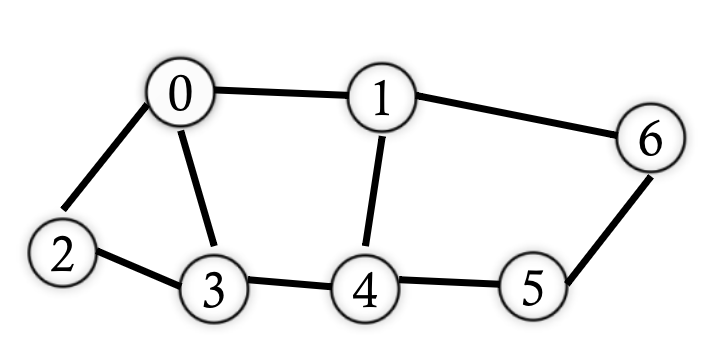
\includegraphics[width=0.5\textwidth,height=\textheight]{images/3.png}
\caption{Example 3}
\end{figure}

\begin{itemize}
\tightlist
\item
  Using a breadth-first traversal, and starting with \(0\): \(\{0\}\)

  \begin{itemize}
  \tightlist
  \item
    Visit all the nodes adjacent to \(0\): \(\{0, 1, 2, 3\}\) (one edge
    away)

    \begin{itemize}
    \tightlist
    \item
      Paths established: \(\{0, 1\}, \{0, 3\}, \{0, 2\}\)
    \end{itemize}
  \item
    Visit neighbors of neighbors: \(\{0, 1, 2, 3, 4, 6\}\)

    \begin{itemize}
    \tightlist
    \item
      Paths established:
      \(\{0, 1\}, \{0, 3\}, \{0, 2\}, \{0, 1, 4\}, \{0, 1, 6\}\)
    \end{itemize}
  \item
    Visit neighbors of neighbors: \(\{0, 1, 2, 3, 4, 6, 5\}\)

    \begin{itemize}
    \tightlist
    \item
      Paths established:
      \(\{0, 1\}, \{0, 3\}, \{0, 2\}, \{0, 1, 4\}, \{0, 1, 6\}, \{0, 1, 4, 5\}\)
    \end{itemize}
  \end{itemize}
\end{itemize}

\begin{longtable}[]{cccc}
\toprule
Node & Prev & Dist & Adjacency List\tabularnewline
\midrule
\endhead
0 & 0 & 0 & 1, 2, 3\tabularnewline
1 & 0 & 1 & 0, 4, 6\tabularnewline
2 & 0 & 1 & 0, 3\tabularnewline
3 & 0 & 1 & 0, 2, 4\tabularnewline
4 & 1 & 2 & 1, 3, 5\tabularnewline
5 & 4 & 3 & 4, 6\tabularnewline
6 & 1 & 2 & 1, 5\tabularnewline
\bottomrule
\end{longtable}

\end{document}
